\documentclass[envcountsame,envcountchap]{svmono}
\usepackage{makeidx}
\usepackage{amsmath}
\usepackage{amsfonts}
\usepackage{amssymb}
\usepackage{graphicx}
\usepackage[bottom]{footmisc}
\usepackage{hyperref}
\usepackage{color}
\usepackage{float}

\hypersetup{colorlinks=true, linkcolor=black, citecolor=black, urlcolor=black}

\makeindex

\author{Hildeberto Mendon\c{c}a}
\title{Yougi}
\subtitle{Managing the Knowledge Produced by the Community}

\begin{document}

\maketitle

\frontmatter

\thispagestyle{empty}
\vspace*{3.5cm}
\begin{flushleft}
Notice: copies of this document may be made for your own use and for distribution to others, provided that you do not charge any fee for such copies and further provided that each copy contains this Copyright Notice, whether distributed in print or electronically.
\end{flushleft}

\tableofcontents

\listoffigures

\listoftables

\mainmatter

\chapter{Introduction}

\section{What is a Community?}

\section{Case Study: Java User Groups}

The chosen case study is based on the personal experience of the team who is developing You. Most of contributions come from the Cear\'{a} Java User Group, which is a technical user group located in the Northeast cost of Brazil. Despite being part of a specific domain, we believe that the proposed model is generic enough to cover the management's needs of most user groups out there.

\subsection{The Java User Group Scenario}

Java User Groups (JUG) are independent and entrepreneur communities of students and professionals around the Java platform and related technologies. They are globally spread with larger concentration in Europe, North America and South America.

Their independence from the industry is particularly interesting because, in general, user groups are promoted by the industry, which is the case of GUG, attached to Google; OUG, attached to Oracle; and MUG, attached to Microsoft.

\subsection{JUGs Around the World}

\subsection{The Need for a Mature User Group Management}

\section{Yougi Mission and Vision}

Yougi is developed by passionate people that are used to do, in a daily basis for several years, what the application does today and what it is planned to do tomorrow for online communities out there. After two years of continuos development, Yougi has consolidated its mission of managing, promoting and spreading knowledge produced by a community of members sharing the same interests and passions.

The project goes beyond services for communities and extends its impact to other areas such as education, economical competitivity and generation of opportunities. Since the application is made available as free and open software, several technical questions from CEJUG's mailing list are actually addressed by examples extracted from Yougi's source code. Beginners and professionals learn how to program and use the platform by studing how the application was developed.

\section{Overview}

\section{Conventions Used in this Book}

Within codes and scripts, when a word is surrounded by '[' it means that word should be replaced by a context-specific value when applied to a particular environment. For example:

\begin{verbatim}
password = [password]
\end{verbatim}

In this case, [password] should be replaced by the real password.

\part{User Guide}

\chapter{Membership Management}

\section{Registration}

The decision to register in the user group always come from the interested person. That is why the only way to add a new member is filling out the initial registration form, accessible through a link in the application header when there is no member logged in. JUG leaders do not have any feature that allow them to add new members manually.

Besides the basic personal data, the registration form also asks the interested person to select one or more of the following options:

\begin{itemize}
\item ``I want to be aware of all events organized and supported by the UG in a local, national and international level'' - as a member, the person will receive information about events organized by the UG (see Chapter \ref{chp:event-management}) and other supported events promoted by partners and sponsors.

\item ``I want to receive sponsors' and supporters' offers of products and services, such as books, courses, magazines, etc'' - only those members who checked this option will be able to participate in raffles, promotions and other contests promoted by sponsors.

\item ``I want to receive local and national job offers related to Java'' - only those members who checked this option will receive job offers from partners and sponsors.

\item ``I want to participate in the technical discussion list'' - checking this option, the member will be automatically registered in the technical mailing list.

\item ``I want to receive news about Java and other related technologies, as well as news about the market and other communities'' - only those members who checked this option will receive news about subjects discussed in the group and other community activities.

\item ``Other UG members will be able to see my profile and contact me directly through the application. The application will carefully protect the email address, not showing it for others'' - only members who checked this option will be able to use the social features of the application.
\end{itemize}

When the interested person submits the registration form, we have to make sure that his/her email address is correct before considering him/her as a member. We send an email message to the email address informed in the form, asking the interested person to confirm their email address by clicking on the confirmation link. This link contains a unique code that guarantees that the link cannot be reused after its first use, confirming the email address only once. The interested person is considered as a member as soon as his/her email address is confirmed. The new member receives a welcome email message and JUG Leaders are informed by email about the successful member registration.

\section{Member Profile}

The member has the right to read and modify any data published on its own profile. The email address is the only data subject of validation. The email validation works the same way it works during the registration: the system sends a message to the new email address with a confirmation code to validate it.

\section{Deactivation}

The deactivation of a member means that he/she will not participate in the activities of the group  starting from the date of the deactivation. No email message, invitation, offer, or any other kind of information will be sent to the deactivated member any longer. Therefore, he/she is not considered as a regular member.

At the same time, all data input by the ancient member in the database will not be removed. Comments, email messages, articles and other information will be kept unchanged indefinitely. Therefore, any modification on these data is not responsibility of the application.

\chapter{Partnership Management}

\section{Registration of Partners}

\section{Sponsorship}

\section{Exclusive Services for Partners}

\subsection{Dissemination of Job Offers}

\subsection{Offers of Products and Services}

\subsection{Search for Talent People}

\chapter{Event Management}
\label{chp:event-management}

Events are strategic for user groups and for companies that want to promote the use of their technology or attract talent people to compose their dream team. The occasion is appropriate to disseminate knowledge and promote networking, strengthening the links between people and increasing the likelihood of new opportunities. Nowadays, there are several ways to build a network virtually, but the body language still is the most efficient way to know people's behaviour, reliability and friendliness. Those good experiences Good ex

It is important to have an efficient event management in order to keep everything under control, measure member's participation and get their feedback.

\section{Event Registration}

To start organizing events, UG Leaders should register venues available and suitable for user group events. A venue might have one or more rooms where event sessions will take place. In case of multiple rooms available, the event can manage multiple sessions in parallel.

Events are allocated in existing venues for a certain time. When an event is registered and allocated to a venue, the venue's contact receives a request email containing details about the event and a list of resources that are expected from them. After a negotiation process the event is confirmed or not. The confirmation occurs when the venue's contact clicks on the confirmation link in the email message. Without this confirmation the event cannot occur.

For each session of the event, one or more speakers may be allocated. A speaker is a qualified person on the subject(s) of the session. He/she is invited by a UG Leader to give a speech, training, coordinate a discussion or any other social activity. The person is invited to register in the application as a speaker.  Once logged in, he/she can put a short summary of his/her experience, an abstract of the session, upload his/her profile picture, presentations, documents, source code, links, and other useful contents for the session. The application will use all this information to compose the page of the event.

When the event is confirmed, an email message containing detailed information is sent to all members that have declared in their registration form the wish to receive information about events. This message contains a direct link to the event registration form.

Detailed information about the event is also formatted to be published on the UG website. Consequently, it may attract people who are interested on the event but are not member of the UG. Those people should become a member of the UG before registering to the event.

Right after the event registration, the member receives a confirmation message just to let him/her know that he/she is successfully registered to attend the event. Registered members will receive a remind email message seven days before the event and a second one on the day before the event. They can cancel their registration at any time before the event.

\section{Controlling the Event}

At the entrance of the event, a member of the UG staff checks the inscription of each person in an available computer. If the person is a member registered in the event, then his/her presence is confirmed. If the person is a member but he/she is not registered in the event, then his/her registration is made at the entrance. If the person is not a member, then he/she should agree to become a member of the UG, otherwise it is not possible to join the event. If he/she agrees to become a member, his/her registration in the UG and in the event is done at the entrance of the event.

\section{After the Event}

When the event has passed, no information about the event can be changed anymore. It will be available only in a read-only mode from the day after. Speakers will not be able to update their profiles either until being allocated to another event. However, UG Leaders are able to publish additional resources related to the event, such as pictures, documents, presentations, etc.

\chapter{Knowledge Management}

\section{Topics}

\section{Mailing Lists from Chaos to Meaningful Content}

\section{Web Content Agregation}

\part{Technical Guide}

\chapter{Architecture}

Yougi should be deployed in an Application Server (AS). This platform is responsible for the system execution, the connectivity to several resources available in the environment and the availability for several users and systems. For the moment, Glassfish 3.1.2 is the standard AS for this application. This JEE Server has gained lots of attention for constantly run towards the state-of-the-art of the Java server side technology. It has an aggressive roadmap, being always the first product on the market to fully implement the last version of the JEE specification.

One of the main advantages of using an application server like Glassfish is to keep the application free of complex code, such as a) manual control of database transactions; b) database access configuration; c) security authentication and authorization; e) sending and receiving e-mail messages, among many other complexities that are non-functional requirements, consuming the time we would be spending on functional requirements.

No test was performed in other AS up to now, mainly because when the project started Glassfish was the only AS implementing the JEE 6 specification (JPA, EJB, JSF, etc.). The AS should have access and provide the following resources:

\begin{itemize}
\item \textit{Database Server}: a database driver allows connections to a relational database and a connection pool manages several simultaneous connections to this database, allowing scalability and performance. MySQL is the database system chosen to organize and protect UG's data.

\item \textit{Email Server}: A JavaMail service connects to an email server and provide sessions to the application, allowing it to send and receive email messages without any special configuration on the implementation side.

\item \textit{Security Realm}: is a provider of authentication and authorization data to identify users who want to access the application and verify whether they have rights to access protected resources.  The application's database, besides storing UG's data, also stores users and their roles, which makes it the realm provider, referenced by Glassfish in the realm configuration.

\item \textit{File System}: the application should be able to save and access files in a specific directory of the file system. Unfortunately, the AS does not manage access to the file system. The application is responsible for managing all uploaded files.
\end{itemize}

The resources provided by the application server help to simplify the overall application architecture. The connectivity with those resources characterizes a n-tier architecture, where each tier is physically separated. The application architecture, in turn, is divided in four layers, as depicted in Figure 1. These layers provide a model to create a flexible and reusable implementation. This way, new features can be efficiently accommodated, with a minimal impact on existing code.

The 4 logical layers are:

\begin{itemize}
\item \textit{View}: implements the user interface by defining the layout of the screens, position UI components, performing data validation (e.g. invalid date format), formatting data to be presented, internationalizing and localizing text, and giving feedback about the user interaction.

\item \textit{Controller}: controls the navigation flow according to the user interaction and intermediates data from the view to the business and vice-versa. It performs business validation (e.g. user already exists), data conversion from user friendly to business model-compliant and vice-versa, accesses business services, creates model objects that do not exist yet and manipulates existing ones. According to the state of the IS, the controller knows which flow should be followed and what to do in case of exceptions and security constraints.

\item \textit{Business}: due to its objectivity, the business layer is not subdivided. It is considered as concrete and it will perform transactional business operations over the data model. Every business operation should guarantee that the data model is consistent before and after its execution. Therefore, the data model can only be access through this layer.

\item \textit{Persistence}: maps data model entities with database tables to manage the lifecycle of entity objects. These objects can be created (insert), updated (update), queried (select) and deleted (delete). These operations are widely used by the data access object layer in order to interact with the database. The persistence layer can manage one or more data sources, but a data source is managed by one and only one data source.
\end{itemize}

\section{Chosen Technologies}

Table \ref{tab:chosen-technologies} lists the technologies adopted by the development team to implement the application.

\begin{table}
\centering
\caption{Chosen technologies to implement logical layers}
\label{tab:chosen-technologies}
\begin{tabular}{lll}
\hline\noalign{\smallskip}
Logical Layer & Technology & Version \\
\noalign{\smallskip}\hline\noalign{\smallskip}
View & JSF Facelets & 2.1 \\
 & Primefaces UI Library & 2.4.2 \\
\noalign{\smallskip}
Controller & Primefaces & 2.1.1 \\
 & JSF Managed Beans & 2.1 \\
\noalign{\smallskip}
Business & EJB Session Beans & 3.1 \\
 & EJB Timer & 3.1 \\
\noalign{\smallskip}
Persistence & JPA & 2.0 \\
 & EclipseLink & 2.0 \\
 & JTA & 1.2 \\
\noalign{\smallskip}\hline
\end{tabular}
\end{table}

These technologies were selected based on the current needs, resources and knowledge of the development team. We decided to adopt a minimalist approach where most libs needed by the application are also distributed with the AS, such as Eclipse Link and Mojarra, and most configurations are made through the Administrative Console, such as database connection pool, JavaMail session and Security Realm. For the moment, the only external lib is the Primefaces component library. We make extensive use of annotations and avoid as much as we can XML for configuration purpose. Transactions are fully managed by the container. This way, we keep focused on the source code of the UG community model. Eventually, other technologies out of this table may be adopted if well justified. Therefore, a new technology would be considered in case a very special UG's need must be fulfilled.

Going into details about the chosen technologies, we describe each one of them, completing the description of Figure 1:

\begin{itemize}
\item \textbf{JSF 2.1}: The Java Server Faces technology is the standard technology for developing web-based applications in the JEE platform.
   \begin{itemize}
   \item \textit{Primefaces}: extensive library of UI Widgets 
   available for the JSF technology.
   \item \textit{Converters}: converts data from user friendly to
   business model-compliant and vice-versa.
   \item \textit{ManagedBeans}: POJO annotated classes that have
   access to special resources available on the
   application context.
   \item \textit{Validators}: performs server-side validation of
   data informed by the user before going forward in the
   controller processing.
   \end{itemize}
\item \textbf{JNDI}: the Java Naming and Directory Service helps to localize and retrieve instances of resources available in the context of the server, reusing existing instances and avoiding the complexity behind creating those instances.
\item \textbf{EJB 3.1}: transactional, distributed and secure component model to encapsulate reusable business logic.
   \begin{itemize}
   \item \textit{Stateless Session Beans}: EJB that does not store
   the state of components in memory, optimizing memory
   allocation and scalability across multiple servers.
   \item \textit{Timer}: EJB capable of scheduling itself to
   execute business logic in a certain time or in a
   certain frequency of time. The schedule of routines is
   very appropriate to perform automatic maintenance
   tasks such as cleaning temporary data, generating
   complex reports, sending alert messages, etc. Timers
   are also useful to efficiently use computational
   resources when systems are in idle mode.
   \item \textit{ManagedBeans}: POJO annotated classes that have
   access to  special resources available on the enterprise
   context.
   \end{itemize}
\item \textbf{JPA 2.0}: Java Persistence API is an entity-relational mapping specification that manages the lifecycle of objects persisted in the database. It reduces the degree of database dependency, the complexity of the source code and the maintenance cost in case of changes in the relational model.
   \begin{itemize}
   \item \textit{Entity Model}: POJO annotated classes mapped to
   database tables where their instances represent table records
   for the business logic.
   \item \textit{JTA}: The Java Transaction API.
   \end{itemize}
\end{itemize}

\section{Database Model}

\begin{figure}
\centering
\includegraphics[height=10cm, angle=90]{figures/relational-model}
\caption{Database relational model}
\label{fig:relational-model}
\end{figure}

\subsection{Liquibase}

To keep the database model up-to-date, Yougi uses the Framework Liquibase\footnote{Liquibase. Database Change Management.  http://www.liquibase.org.}. This framework empowers the application to update the database during deployment time. It simplies the upgrade of the application, reducing it to a simple deployment.

During development time, if the database needs to change, the developer should add change sets to one or several xml files located in the module yougi-web, at src/main/resources/org/cejug/yougi/db/changelog.

\chapter{Installation}
\label{chp:installation}

To install Yougi we need:

\begin{itemize}
\item Java Standard Edition JDK 7;
\item Glassfish 3.1.2 Server or superior;
\item MySQL 5 or superior;
\item MySQL ConnectorJ JDBC Driver;
\item Access to a SMTP and POP 3 server to send and receive email messages.
\end{itemize}

The initial installation takes some time, but it will guarantee easy updates when new releases come out. Because the installation of Java SE JDK, Glassfish and MySQL are dependent on the target platform, we consider that they were already performed by the administrator, who knows details about the hosting system. We would not be complete and up-to-date enough to cover all the possibilities, thus the best source of information is their respective websites. 

The steps to install the application are:

\begin{enumerate}
\item Create a MySQL database: run SQL scripts to create a database and its structure dedicated for the application. The last available version of the database script is mysql-create.sql.
\item Install the JDBC Driver on Glassfish: make the MySQL ConnectorJ JDBC Driver available in the application server classpath to be used by the connection pool to create new MySQL database connections.
\item Create a database connection pool on Glassfish: the connection pool manages connections to the database using the JDBC Driver.
\item Create a datasource for the connection pool on Glassfish: the datasource links the connection pool to the application. In other words, the connection pool is a resource and the datasource is a name for this resource. This name is used in the application to locate and use that resource.
\item Create a JavaMail session: since this application deals with people, it has to send emails very often. Therefore, the availability of a JavaMail session, managed by the container, is essential to support the high demand for sending and receiving emails without dealing with the complexity of managing email server connections.
\item Create a Security Realm: the security realm allows the declarative implementation of the application's security, significantly reducing the application complexity by delegating this responsibility to the container.
\item Deploy the application package: finally, we deploy the application package that makes use of all configurations above.
\item Configure the application according to specific needs of the community: after the initial deployment the application will run normally using default configuration. However, the application will be fully operational only when specific configurations for the community are defined. For instance: there will not be no location registered at the beginning and they have to be created to allow the registration of new members.
\end{enumerate}

\section{Creating the MySQL Database}

Yougi has access to only one database. This database is created using the Administrative Console and a SQL script. As mentioned before, this instructions consider that the MySQL database, version 5.0 or superior, is already installed and configured. In terms of configuration, we also consider that the path of the operating system is pointing to the folder where all MySQL commands are located.

The procedure starts executing the console, using the following command:

\begin{verbatim}
# mysql -u root -p
\end{verbatim}

Usually, an administrative user is needed to create a new database. The user \textit{root} is the one with privileges to perform this operation. It will create a client authenticated session to access MySQL. \textit{-u} means that the subsequent value is the user of the session and \textit{-p} means that the password should be prompted right after executing the command. Once authenticated, the user \textit{root} will allow the execution of the command below, which creates the database and a dedicated user for it:

\begin{verbatim}
mysql> create database ug;
mysql> create user 'ug_user'@'localhost' identified by '[password]';
mysql> use ug;
mysql> grant all privileges on ug.* to 'ug_user'@'localhost';
mysql> flush privileges;
\end{verbatim}

The database \textit{ug} and the user \textit{ug\_user} are created, and all privileges over the \textit{ug} database are granted to the \textit{ug\_user}. To check if the database was created, execute the following command:

\begin{verbatim}
mysql> show databases;
\end{verbatim}

Check if the database \textit{ug} is in the list. If necessary, you can drop the user to create it again:

\begin{verbatim}
mysql> drop 'ug_user'@'localhost';
\end{verbatim}

Or you can reset the password:

\begin{verbatim}
mysql> set password for 'ug_user'@'localhost' = password('[password]');
\end{verbatim}

To leave the MySQL command prompt, use the command \textit{quit}.

\begin{verbatim}
mysql> quit;
\end{verbatim}

The user \textit{ug\_user} and its password should be used in the configuration of the connection pool. Do not use the \textit{root} user for application purposes.

\section{Installing the JDBC Driver on Glassfish}

The driver installation consists on saving the driver file in a specific AS lib directory. For this step we consider that Glassfish AS, version 3.1 or superior, is already installed and configured. The driver is available to download at MySQL's website (http://www.mysql.com). The downloaded file contains the driver and its documentation. Copy  the driver file mysql-connector-java-[version]-bin.jar to the directory /glassfish/domains/domain1/lib/. The server needs to be restarted to make the driver available.

\section{Creating a Database Connection Pool}
\label{sec:creating-database-connection-pool}

The database connection pool is managed by the AS. There are many ways to create a connection pool. We are going to show two possibilities: changing configuration files directly and using the Administrative Console.

To create the database connection pool through the configuration file, open the file [glassfish\_home]/glassfish/domains/domain1/config/domain.xml. Go to the element \textless resources\textgreater \ and add the following connection pool and jdbc resource under the last closing \textless /jdbc-connection-pool\textgreater \ element.

\begin{verbatim}
<resources>
   ...
   </jdbc-connection-pool>
   <jdbc-connection-pool driver-classname="" datasource-classname=
       "com.mysql.jdbc.jdbc2.optional.MysqlConnectionPoolDataSource"
       res-type="javax.sql.ConnectionPoolDataSource" description="" 
       name="UGPool" ping="true">
         <property name="User" value="ug_user"/>
         <property name="DatabaseName" value="ug"/>
         <property name="Password" value="[password]"/>
         <property name="ServerName" value="localhost"/>
         <property name="PortNumber" value="3306"/>
   </jdbc-connection-pool>
   <jdbc-resource pool-name="UGPool" description="" 
                  jndi-name="jdbc/ug"/>
</resources>
\end{verbatim}

Now, find the element \textless server name=''server'' config-ref=''server-config''\textgreater \ and put inside the following line after the latest \textless /resource-ref\textgreater element:

\begin{verbatim}
<server name="server" config-ref="server-config">
   ...
   <resource-ref ref="jdbc/ug"/>
</server>
\end{verbatim}

If you prefer to do it in the Administrative Console, you can go through the following steps:

\begin{enumerate}
\item  Enter in the Administrative Console at http://[servername]:4848/ and navigate to Resources / JDBC / Connection Pools.
\item Create a new connection pool with the name UGPool, select the resource type javax.sql.ConnectionPoolDataSource, select the database vendor MySQL and click next.
\item Select the datasource classname \\ \textit{com.mysql.jdbc.jdbc2.optional.MysqlConnectionPoolDataSource} and inform the following additional properties:
   \begin{enumerate}
   \item DatabaseName=ug
   \item User=ug\_user
   \item Password=[password]
   \item PortNumber=3306 (this is the default port but make sure
   that you are using the correct one)
   \item ServerName=[server-name or ip address]
   \end{enumerate}
\item Click on \textit{Finish} to save the new connection pool.
\item Go to the list of connection pools again and select the new one that was just created.
\item Click on \textit{Ping} to check if the connection was correctly configured. The message "Ping Succeeded" means that the connection is working fine and ready for use.
\end{enumerate}

Now, we create a JNDI name for it at \textit{Resources/JDBC/JDBC Resources}.

\begin{enumerate}
\item Click on \textit{New} to start the creation of the data source.
\item Set the field \textit{JNDI Name} to \textit{jdbc/ug}.
\item Select the connection pool \textit{UGPool} (see section \ref{sec:creating-database-connection-pool}).
\item Click \textit{Ok} to finish.
\end{enumerate}

The only information the application knows about the database is the jdbc resource jndi name, which is ''jdbc/ug''. This is important because the application should not contain any security related data, such as database's username and password. We should let the server administrator define these configuration on the server, according to his security principles.

\section{Creating a JavaMail Session}

Besides managing the connections to the email server, the JavaMail session stores security parameters, such as user name, password, SSL, the kind of server available and so on. These parameters are defined in a case by case basis, thus the JavaMail service provided by the application server is essential for the distribution of this application.

You can configure JavaMail directly in the domain.xml file, by copying and pasting the xml below after the element \textless jdbc-resource\textgreater, and then change the values according to your email server.

\begin{verbatim}
<resources>
   ...
   </jdbc-connection-pool>
   <jdbc-resource pool-name="UGPool" description="" 
                  jndi-name="jdbc/ug"/>

   <mail-resource host="[smtp_server_name]" description="" 
                  jndi-name="mail/ug" from="[your@emailaddress]"
                  user="smtp_user">
      <property name="mail.smtp.port" value="[port_number]"/>
      <property name="mail.smtp.auth" value="true"/>
      <property name="mail.smtp.password" value="[password]"/>
      </property>
   </mail-resource>
</resources>
\end{verbatim}

Add the element \textless resource-ref\textgreater \ of this new resource after the resource-ref created for the connection pool, as illustrated below:

\begin{verbatim}
<server name="server" config-ref="server-config">
   ...
   <resource-ref ref="jdbc/ug"></resource-ref>
   <resource-ref ref="mail/ug"></resource-ref>
</server>
\end{verbatim}

To configure JavaMail using the Administrative Console, follow the steps below:

\begin{enumerate}
\item Enter in the Administrative Console (http://[server-name]:4848/).
\item Go to \textit{Resources / JavaMail Sessions}.
\item create a new JavaMail session and set the following properties:
   \begin{enumerate}
   \item JNDI Name: mail/ug
   \item Mail Host: [smtp-server-name]
   \item Default User: the username to authenticate on the smtp
    server
   \item Default Return Address: the address used by recipients to
    reply the message. Some servers require that this address
    should be the one used by the authenticated user to access his
    mailbox.
   \end{enumerate}
\end{enumerate}
 
If the server doesn't request secure authentication, then the three steps above are enough to start using the new JavaMail session, but a server without secure authentication is a very rare case nowadays. Therefore, we will certainly need to inform a password to login on the smtp server. In most cases, the server administrator also changes the default port of the smtp server, which forces us to explicitly inform the correct port. For these special needs we can use additional properties in the JavaMail session. Follow the steps below:

\begin{enumerate}
\item Still on the JavaMail session form, go to the \textit{Additional Properties} section and add 3 more properties, which are:
   \begin{enumerate}
   \item mail.smtp.port: [port-number]
   \item mail.smtp.auth: true
   \item mail.smtp.password: [password]
   \end{enumerate}
\item Click on \textit{Save} to create the JavaMail session.
\end{enumerate}

More supported JavaMail properties can be found on Table \ref{tab:javamail-properties} in the Appendix.

\section{Creating a Security Realm}

A realm is a security policy domain available on Glassfish to provide authentication and authorization services for web applications. A realm contains a collection of users and their assignements to groups and roles.

As the connection pool and the JavaMail session, the security realm is also a configuration entirely made in the application server. Since Yougi's users are stored in the database, we have to use a realm based on JDBC. The JDBC Realm uses the data source created in section \ref{sec:creating-database-connection-pool} to access users' data on Yougi's database.

As usual, we start with the fastest configuration option, by directly changing the domain.xml file. Copy and paste the xml below within the element \textless security-service\textgreater .

\begin{verbatim}
<security-service>
   ...
   <auth-realm name="ug-realm"
       classname="com.sun.enterprise.security.auth.realm.jdbc.JDBCRealm">
       <property name="jaas-context" value="jdbcRealm"/>
       <property name="encoding" value="Base64"/>
       <property name="user-table" value="authentication"/>          
       <property name="password-column" value="password"/>
       <property name="datasource-jndi" value="jdbc/ug"/>
       <property name="group-table" value="user_group"/>
       <property name="group-name-column" value="group_name"/>
       <property name="group-table-user-name-column" value="username"/>
       <property name="digest-algorithm" value="SHA-256"/>
       <property name="user-name-column" value="username"/>
   </auth-realm>
   ...
</security-service>
\end{verbatim}

If you prefer, you can always use the Adminstrative Console to configure the JDBC Realm. Just follow the steps below:

\begin{enumerate}
\item Enter in the Administrative Console (http://[server-name]:4848).
\item Go to \textit{Configuration/server-config/Security/Realms}, press \textit{New...} and inform the following values:
   \begin{enumerate}
   \item Name: ug-realm
   \item Class Name: com.sun.enterprise.security.auth.realm.jdbc.JDBCRealm
   \item JAAS Context: jdbcRealm
   \item JNDI: jdbc/ug - the data source JNDI name pointing to the connection pool where user data are available
   \item User Table: authentication
   \item User Name Column: username
   \item Password Column: password
   \item Group Table: user\_group
   \item Group Table User Name Column: username
   \item Group Name Column: group\_name
   \item Digest Algorithm: SHA-256
   \item Encoding: Base64
   \end{enumerate}
\item Restart the application server to activate the realm.
\end{enumerate}

\section{Deploying the Application Package}

The installation process takes some time, but all these steps are executed only once, simplifying significantly the development process by going from development to test and production without any specific application customization. The deployment process is also simplified, reducing this final phase, as follows:

\begin{enumerate}
\item enter in the Administrative Console (http://[server-name]:4848).
\item Go to \textit{Applications} and press \textit{Deploy...}.
\item Inform the package \textit{yougi.ear} to be uploaded to the server.
\item Select type \textit{Enterprise Application}.
\item Click \textit{Ok} to deploy.
\item Check if everything went well accessing http://localhost:8080/ug if deploying on your own computer or http://[servername]:8080/ug if deploying on the server.
\end{enumerate}

Yougi will appear in the list of applications. In case of updating an application already deployed, the process is very simplified because of the initial configuration:

\begin{enumerate}
\item enter in the Administrative Console (http://[server-name]:4848).
\item Go to \textit{Applications}.
\item click on the action \textit{Redeploy} in the row of the yougi application;
\item inform the package “yougi.ear” to be uploaded to the server; and
\item click \textit{Ok} to redeploy.
\item Check if everything went well accessing http://[server-name]:8080/ug.
\end{enumerate}

\section{Configuring the Application}

Before using the application, the database should be initialized with some initial data that are specific for each UG. The following steps are necessary:

\begin{enumerate}
\item registration of the administrative user: after the initial deployment, there is no user registered in the application. Even the administrator is not present. When the user tries to authenticate while there is no registered user, the navigation redirects him/her to the registration page. On the top of the form, the user is alerted that he/she is going to be the first member and will be considered as administrator. The form is a simplified version of the original registration form because some mandatory data are not available yet, such as geographic location. As an initial user, he/she is automatically confirmed, without the need of a confirmation by email.
\item definition of the UG location and geographic coverage: because country and city are mandatory fields in the registration form for all other users, the administrator should define them as soon as he/she have access to the application. The administrator should register at least a country to allow the registration of members, but it is expected from him/her that the location of the UG and its coverage are also registered. It means that the administrator should register all countries, provinces and cities where the UG has influence.
\item definition of application properties: at last, but not least, the administrator should review and modify, if needed, the default value of application properties. This properties are initialized in a way that allows the application run normally. However, some properties are missing by default and others might be different from what is expected.
\end{enumerate}

\chapter{Development}

As explained in the previous chapter, it is not necessary to start from the source code to install and use Yougi. The binary package is available at http://yougi.org/downloads. On the other hand, if the intention is to contribute to the project, a set of other actions are necessary. A potential contributor may:

\begin{itemize}
\item Be pationate about open source initiatives and technologies.
\item Be interested in learning Enterprise Java technologies.
\item Be excited about implementing a solution to manage comunities.
\item Learn JavaEE, Maven, Arquillian, JUnit, and other technologies used in the project.
\end{itemize}

If you fell confortable with these principals, this chapter will help you to get started, explaining how to contribute to the source code of the project.

\section{Preparing the Development Environment}

Before starting, make sure you have everything it takes to develop Yougi. Basically, you have to:

\begin{itemize}
\item Install and configure Git, a version control system used to manage the source code and its distribution.
\item Create an account on Github and learn the social aspect of it.
\item Install and configure a Java IDE, preferably Netbeans because it is one of the best IDEs available to work with JavaEE applications.
\item Install and configure an application server, preferably Glassfish, which is probably the more mature Java EE implementation available.
\item Install and configure a relational database,  
\end{itemize}

\subsection{Obtaining the Source Code}
\label{ssec:obtaining-source-code}

Git is the version control system (VCS) used to control Yougi source code. For being a distributed VCS, Git is not that trivial. Its foundations are a bit different from traditional VCSs, such as CVS and SVN. So, you have to rethink some concepts while working with Git. We will explore the necessary here, but it is always good to master it later through books, training and other means.

The master repository is located at http://github.com/htmfilho/yougi, where the main trunk (master) is centralized, but every client is also a full featured VCS, where is possible to perform commits off line, create branches and merge with other clients without acknowledging the master.

fork the main repository

clone your own fork to your computer.

\begin{verbatim}
#git config --global user.name "John Smith"
#git config --global user.email "john.smith@gmail.com"

# mkdir yougi
# cd yougi
# git clone https://github.com/[your-github-username]/yougi.git .
\end{verbatim}

\subsection{Building the Project for the First Time}

Start Netbeans

Open Maven project: yougi

Clean and Build: yougi

\begin{verbatim}
-------------------------------------------------------------
Reactor Summary:

yougi ..................................... SUCCESS [6.170s]
yougi-ejb  ................................ SUCCESS [37.864s]
yougi-web  ................................ SUCCESS [34.020s]
yougi-ear  ................................ SUCCESS [5.009s]
-------------------------------------------------------------
BUILD SUCCESS
-------------------------------------------------------------
Total time: 1:23.555s
Finished at: Sun May 05 17.45.48 CEST 2013
Final Memory: 28M/369M
-------------------------------------------------------------
\end{verbatim}

Freely change the files in your local clone, trying to solve one of the issues reported at: https://github.com/htmfilho/yougi/issues.

Add the changed files to the stage for commit

\begin{verbatim}
git add [file]
\end{verbatim}

Only add files that should be committed.



\begin{enumerate}
\item install Git in the development machine: the installation is dependent of platform, thus the instructions for the target platform are only available on the Git website: http://git-scm.com.
\item configure Git to access the master repository: Yougi's Git accepts only secure SSH (Security Shell protocol) connection, making the initial steps more complicated than expected. After this initial configuration, the access to the master becomes transparent and secure.
\item register at github.com.
\item copy and paste the public key in your Github personal profile.
\item register yourself as a member of the CEJUG Community at \\ http://cejug.org/ug/registration.xhtml. You will have access to the repository only if you are a CEJUG member.
\end{enumerate}

To make sure that the code in the server branch is perfectly working, we have to update the local copy with the latest changes available on the server, test the system locally with those changes and if everything is working well, the local commits can finally be pushed to its respective branch. Before updating the local, make sure that there is no pending commit using:
\begin{verbatim}
# git status
\end{verbatim}
If there are changed files add them using:
\begin{verbatim}
# git add [file]
\end{verbatim}
Use the command above for each modified file or if they all make sense to be committed together use:
\begin{verbatim}
# git commit -a -m [message]
\end{verbatim}
to add all changed files and commit right after. If files were added individually use:
\begin{verbatim}
# git commit -m [message]
\end{verbatim}

After performing the last commits, it is time to update the local copy using:
\begin{verbatim}
# git pull
\end{verbatim}
or
\begin{verbatim}
# git fetch
# git merge FETCH_HEAD
\end{verbatim}

Note that the pull is done after all commits. It was put on this sequence on purpose because the pull will try to merge the version on the server with the local version, but it can only happen if the files were committed. If there is nothing to merge, then there is no problem, but if something needs to be merged then a problem will occur during the pull operation. Therefore, it is always recommended to commit all local changes before updating the local version. In case you didn't seriously changed your files and don't want to commit those changes, you can discard them, by performing the following command for each changed file:

\begin{verbatim}
#git checkout -- [file]
\end{verbatim}

To push local commit to the server, use:

\begin{verbatim}
#git push origin master
\end{verbatim}

\begin{figure}
\centering
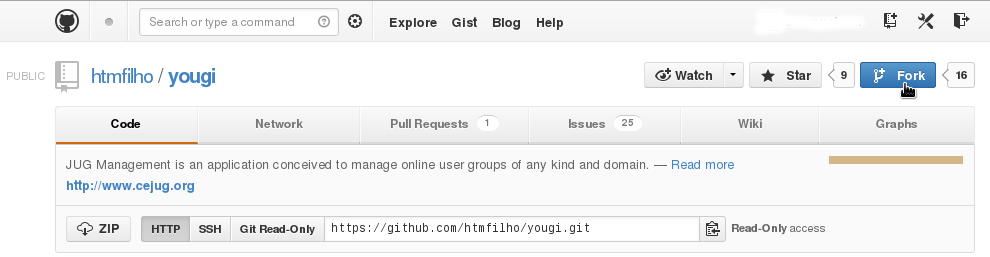
\includegraphics[scale=.34]{figures/github-fork}
\caption{Forking the main repository}
\label{fig:github-fork}
\end{figure}

It is a good practice to refresh your fork before creating a pull request. It will substantially reduce the effort of the committers while trying to merge your contributions. The main trunk might have been under intense changes, made by different people in parallel, and refreshing your fork is also a way to also distribute the effort of having the application more stable and complete.

Go to your own fork page and you will see the possibility of creating a pull request to the original repository. The commits you have done to your own repository will be in the scope of the pull request. There are some fields available to allow you to explain in details what you have done. This is very important because in a distributed team we don't have the chance to talk in person and things turn to be more difficult to understand. Figure \ref{fig:github-pull-request-example} shows an example of a pull request that is about to be sent.

\begin{figure}
\centering
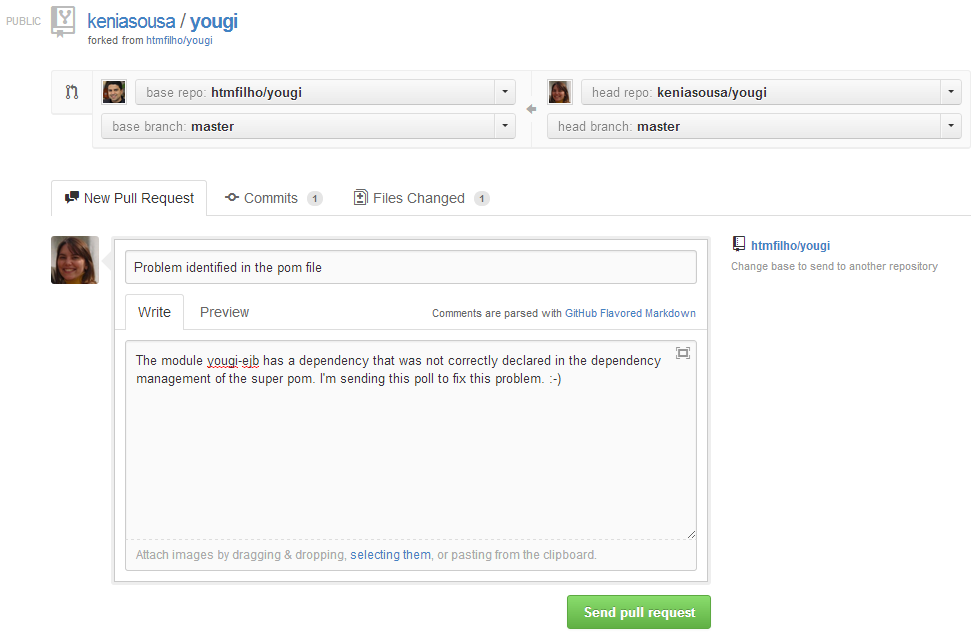
\includegraphics[scale=.46]{figures/github-pull-request-example}
\caption{Example of pull request}
\label{fig:github-pull-request-example}
\end{figure}

The pull request appears in the main repository and any of the existing committers can take the initiative to review and approve/desaprove it, as illustrated in Figure \ref{fig:github-pull-request-merged-closed}.

\begin{figure}
\centering
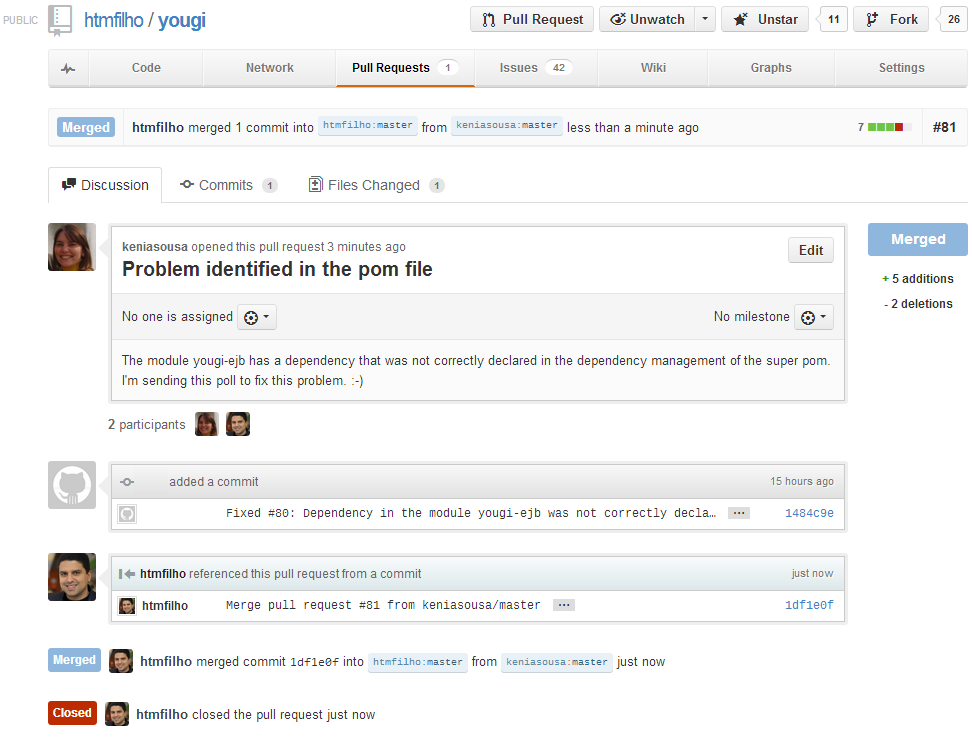
\includegraphics[scale=.46]{figures/github-pull-request-merged-closed}
\caption{Review and approval of the received pull request}
\label{fig:github-pull-request-merged-closed}
\end{figure}

\subsection{Configuring the Eclipse IDE}

Eclipse is the most popular Java IDE. Since it is, basically, a multi-purpose platform, Eclipse should be suficiently extended to allow productive development of a JavaEE application, such as Yougi. In this section we will work with Eclipse Juno (4.2). It is available for download at: http://eclipse.org/downloads.

We start extending Eclipse to work with Git (read Section \ref{ssec:obtaining-source-code} for more details about Git):
\begin{enumerate}
\item On the menu, select Help / Install New Software.
\item In the new dialog, select the option \textit{Juno - http://download.eclipse.org/releases/juno} in the combobox to see several plugins available for the current Eclipse version.
\item In the filter, type ''git'' to find the plugin that supports Git.
\item Follow the installation procedure.
\item Restart the IDE when finished.
\end{enumerate}

The next step is to import the project into Eclipse:
\begin{enumerate}
\item On the menu, select File / Import / Git / Project From Git / URI
\item Inform the URI https://github.com/htmfilho/yougi and click on ''Next'' twice.
\item Inform the directory where you want to import the project and click on ''Next''.
\item Select the option ''Import General Project''.
\item Click on ''Next'' and then finish.
\end{enumerate}

Figure \ref{fig:eclipse-project-opened} shows how the project looks like after the import. 

\begin{figure}
\centering
\includegraphics[scale=.7]{figures/eclipse-project-opened}
\caption{The project opened in the Eclipse IDE}
\label{fig:eclipse-project-opened}
\end{figure}

\part*{Appendix}

\chapter*{JavaMail Properties}

Table \ref{tab:javamail-properties} lists all relevant JavaMail properties.

\begin{table}
\centering
\caption{Complete list of JavaMail properties}
\label{tab:javamail-properties}
\begin{tabular}{lll}
\hline\noalign{\smallskip}
Name & Type & Description  \\
\noalign{\smallskip}\hline\noalign{\smallskip}
mail.smtp.user & String & Default user name for SMTP. \\
mail.smtp.host & String & The SMTP server to connect to. \\
mail.smtp.port & int & The SMTP server port to connect to.\\ & & Defaults to 25. \\
mail.smtp.connectiontimeout & int & Socket connection timeout value in \\ & & milliseconds. Default is infinite timeout.\\
mail.smtp.timeout & int & Socket I/O timeout value in milliseconds. \\ & & Default is infinite timeout. \\
mail.smtp.from & String & Email address to use for SMTP MAIL \\ & & command. This sets the envelope return \\ & & address. Defaults to msg.getFrom() or \\ & & InternetAddress.getLocalAddress(). \\
mail.smtp.ssl.enable & boolean & If set to true, use SSL to connect and use \\ & & the SSL port by default. Defaults to false \\ & & for the "smtp" protocol and true for the \\ & & "smtps" protocol. \\
mail.smtp.starttls.enable & boolean & If true, enables the use of the STARTTLS\\ & & command (if supported by the server) to\\ & & switch the connection to a TLS-protected\\ & & connection before issuing any login\\ & & commands. Defaults to false. \\
mail.smtp.starttls.required & boolean & If true, requires the use of the STARTTLS \\ & & command. If the server doesn't support the \\ & & STARTTLS command, or the command \\ & & fails, the connect method will fail. \\ & &Defaults to false. \\
\noalign{\smallskip}\hline
\end{tabular}
\end{table}

\backmatter

\printindex

\begin{thebibliography}{99.}
\end{thebibliography}

\end{document}